\chapter{Reziduálne neurónové siete}

\label{ResNet_kap2}

Hlboké siete je náročné trénovať. Nedávny výskum ukázal, že hĺbka neurónovej siete má zásadný vplyv na presnosť neurónovej siete \cite{Wu2017, He2016, Targ2016}. Ako sme uviedli v Kapitole \ref{synth_grad}, učenie neurónovej siete predstavuje úpravu váh jednotlivých vrstiev za účelom minimalizovania hodnoty chyby na výstupe neurónovej siete. Vo fáze spätného šírenia chyby, sa na úpravu váh používa gradient šírený spätnou propagáciou chyby. Pri využívaní spätne šíreného gradientu v prípade veľmi hlbokých neurónových sieti nastáva jav zvaný \textit{miznúci gradient}.
Tento jav brzdí konvergenciu presnosti neurónovej siete už od začiatku etapy trénovania \cite{Wu2017}. Hlboké neurónové siete majú tendenciu znehodnocovať užitočné dáta \cite{Targ2016}. Miznúci gradient spôsobuje, že prvé vrstvy nadobudnú pozitívne vlastnosti a sú schopné poskytovať užitočné dáta. Tieto dáta sú ďalšími transformáciami znehodnotené natoľko, že posledné vrstvy hlbokej neurónovej siete obdržia už neužitočné dáta \cite{Wu2017}.

Problém miznúceho gradientu je význačný tým, že akonáhle je hlboká neurónová sieť schopná začať konvergovať, nastáva rapídna degradácia presnosti. Vo fáze trénovania za ideálnych podmienok presnosť neurónovej siete konverguje k hodnote 100\%. V prípade \textit{miznúceho gradientu} však nedochádza k tejto konvergencii ale priebeh trénovania je sprevádzaný saturáciou presnosti a následnou rapídnou degradáciou. Tento problém nie je spôsobený preučením neurónovej siete ale zvýšeným počtom skrytých vrstiev, ktorý vedie k nárastu chyby neurónovej siete \cite{Wu2017}. 

Nie všetky modely neurónových sietí je možné optimalizovať rovnakým spôsobom \cite{Wu2017}. Na riešenie tohto problému sa používajú dodatočné prepojenia poskytujúce \textit{identické zobrazenie}. Tieto vrstvy sa nazývajú \textit{identitné prepojenia} \cite{Wu2017, Targ2016}. Identitné prepojenia umožňujú jednotlivým vrstvám šírenie dát naprieč neurónovou sieťou bez útlmu, ktorý je spôsobený vykonaním viacerých nelinárných transformácii \cite{Targ2016}. Identické zobrazenie môže byť poskytnuté každej vrstve neurónovej siete samostatne alebo tiež skupine viacerých vrstiev. Tieto vrstvy, ktorým prislúcha samostatné identitné prepojenie sa nazývajú \textit{kumulované vrstvy}. Kumulované vrstvy spolu s identitným prepojením vytvárajú \textit{reziduálny blok}. Skupina zjednotených, serializovaných reziduálnych blokov tvorí reziduálnu sieť, \textit{ResNet} (z angl. Residual Network, ďalej len ResNet).

ResNet predstavuje neurónovú sieť ktorá na generovanie identického zobrazenia namiesto priameho zobrazenia $x\rightarrow y$ pomocou funkcie $\mathcal{H}(x)$ (pozostávajúcej z niekoľkých nelineárnych vrstiev), využíva reziduálne bloky \cite{Wu2017}. Tieto reziduálne bloky sú definované ako funkcia $\mathcal{F}(x) = \mathcal{H}(x) - x$. Pôvodné zobrazenie môžeme prepísať ako $\mathcal{H}(x) = \mathcal{F}(x) + x$, kde $\mathcal{F}(x)$ predstavuje reziduálne zobrazenie (transformáciu kumulovanými vrstvami daného reziduálneho bloku) a $x$ je identické zobrazenie. Pre neurónovú sieť je jednoduchšie optimalizovať reziduálne zobrazenie $\mathcal{F}(x)$ poskytnuté reziduálnym blokom, ako optimalizovať pôvodné zobrazenie $\mathcal{H}(x)$ \cite{Wu2017}.

V ďalších častiach tejto kapitoly uvedieme spôsoby akými sa reziduálne siete trénujú a priblížime si transformáciu identického zobrazenia šíreného reziduálnou sieťou. Zameriame sa na možnosti implementácie reziduálnej siete a na ich vplyv na celkovú presnosť trénovaného modelu.

\section{Reziduálne učenie}
\label{residual_learning}

Reziduálna sieť je architektúra neurónovej siete, ktorá je prispôsobená na generovanie identického zobrazenia. Reziduálna sieť je realizovaná klasickou doprednou neurónovou sieťou, ktorá má jednotlivé vrstvy alebo skupiny vrstiev prepojené identitnými prepojeniami \cite{Wu2017}. Vrstvy ktoré disponujú vlastným identitným prepojením (kumulované vrstvy), transformujú vstupné dáta $x$ funkciou $\mathcal{F}(x)$ (viď Obrázok \ref{fig:residualBlock}). Transformované dáta $\mathcal{F}(x)$ sa na výstupe reziduálneho bloku sčítavajú s identickým zobrazením $x$ ako $\mathcal{F}(x)+x$. Takto upravené dáta sa odosielajú ďalšiemu reziduálnemu bloku, ktorý ich prijímajú ako identické zobrazenie. Identitné prepojenia nepridávajú dátam žiadne dodatočné parametre a nemenia celkovú výpočtovú zložitosť. Trénovanie reziduálnej siete je realizované spätnou propagáciou chyby \cite{Wu2017}.

\begin{figure}

%vlozenie samotneho obrazku vycentrovaneho a vhodnej velkosti
%obrazok je v subore images/cervik.png
\centerline{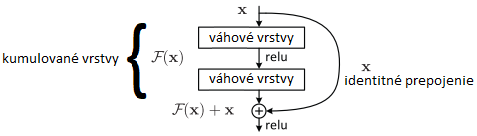
\includegraphics[width=0.8\textwidth]{images/residualBlock}}
%popis obrazku
\caption[Reziduálny blok]{Reziduálny blok pozostávajúci z dvoch kumulovaných vrstiev, ktoré nad vstupnými dátami $x$ vykonávajú transformáciu $\mathcal{F}(x)$. Transformované dáta sa následne sčítavajú s identickým zobrazením $x$ ako $\mathcal{F}(x) + x$ \cite{Wu2017}.}
\label{fig:residualBlock}
%id obrazku, pomocou ktoreho sa budeme na obrazok odvolavat
\end{figure}

Zdroj \cite{Wu2017} uviedol hypotézu, v ktorej tvrdí, že ak viaceré nelineárne vrstvy sú schopné asymptoticky aproximovať zložité funkcie, tak je tiež možné asymptoticky aproximovať aj reziduálne funkcie (ako napríklad $\mathcal{H}(x) - x$). Lepšie než očakávať že jednotlivé vrstvy neurónovej siete budú schopné aproximovať funkciu identického zobrazenia $\mathcal{H}(x)$ je, nechať ich aproximovať reziduálnu funkciu $\mathcal{F}(x) = \mathcal{H}(x) - x$ \cite{Wu2017}. Podľa hypotézy je možné obe tieto funkcie asymptoticky aproximovať, no zložitosť procesu môže byť v oboch prípadoch rozdielna.

Jednoduchšie je naučiť reziduálny blok predikovať identické zobrazenie, než to naučiť viacero vrstiev jednoduchej neurónovej siete (viď Obrázok \ref{fig:plainNetVsResNet}). Ak je obdržané identické zobrazenie optimálne, tak na predikciu identického zobrazenia stačí aby kumulované vrstvy generovali nulové zobrazenie, $\mathcal{F}(x)=0$ \cite{Wu2017}. Tento proces je podstatne jednoduchší ako trénovanie modelu na aproximáciu funkcie $\mathcal{H}(x)$, ktorá predikuje identické zobrazenie len za použitia viacerých nelineárnych vrstiev. V skutočnosti je veľmi nepravdepodobné, že identické zobrazenia obdržané reziduálnymi blokmi sú optimálne. V každom prípade, reziduálna sieť, identické zobrazenia šírene medzi reziduálnymi blokmi za optimálne považuje.

\begin{figure}

%vlozenie samotneho obrazku vycentrovaneho a vhodnej velkosti
%obrazok je v subore images/cervik.png
\centerline{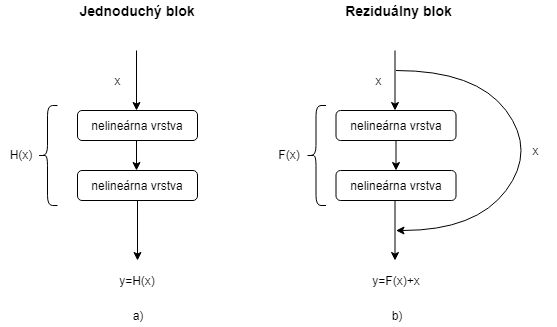
\includegraphics[width=0.8\textwidth]{images/plainNetVsResNet}}
%popis obrazku
\caption[Porovnanie jednoduhcého a reziduálneho bloku]{a) Jednoduchý blok ktorý na predikciu identického zobrazenia využíva len nelineárne vrstvy. Použitím niekoľkých nelineárnych vrstiev je podstatne náročnejšie získať funkciu $\mathcal{H}(x)=x$, ktorá predikuje identické zobrazenie $y=x$ ako $y=\mathcal{H}(x)$. b) Reziduálny blok využívajúci identitné prepojenie na predikciu identického zobrazenia. Oproti jednoduchému bloku je v tomto prípade jednoduchšie získať funkciu $\mathcal{F}(x)=0$ ktorá poskytuje indentické zobrazenie $y=x$ ako $y=\mathcal{F}(x)+x$ \cite{Wu2017}.}
\label{fig:plainNetVsResNet}
%id obrazku, pomocou ktoreho sa budeme na obrazok odvolavat
\end{figure}

Zdroj \cite{Wu2017} uviedol experiment, v ktorom porovnal presnosť predikcie jednoduchej neurónovej siete s 18 skrytými vrstvami, jednoduchej neurónovej siete s 34 skrytými vrstvami, reziduálnej siete s 18 skrytými vrstvami a reziduálnej siete s 34 skrytými vrstvami. Všetky tieto neurónové siete boli trénovanie na rozpoznávanie obrazu z dátovej sady CIFAR-10.

Podľa výsledkov experimentu, pridávanie dodatočných skrytých vrstiev do jednoduchej neurónovej siete spôsobuje degradáciu presnosti danej neurónovej siete. V prípade výskytu degradácie presnosti má jednoduchá neurónová sieť, využívajúca viaceré nelineárne vrstvy, značné problémy s predikciou identického zobrazenia \cite{Wu2017}. Presnosť reziduálnych sieti sa nezmenila ani dodatočným pridaním ďalších skrytých vrstiev. Pridaním identitných prepojení je neurónová sieť schopná aproximovať identické zobrazenie s nižšou hodnotou chyby ako v prípade jednoduchej siete \cite{Wu2017}.

\section{Možnosti implementácie reziduálnych sieti}
\label{implementation}

Reziduálny blok je hlavná stavebná a výpočtová jednotka reziduálnych sieti. Práve vďaka týmto blokom sa reziduálna sieť líši od iných neurónových sieti. Primárnou funkciou týchto reziduálnych blokov je predikcia identického zobrazenia. Jednotlivé reziduálne bloky na predikciu identického zobrazenia využívajú transformačnú funkciu $\mathcal{F}(x)$ ktorá je realizovaná niekoľkými nelineárnymi vrstvami a identické zobrazenie $x$, obdržané z predchádzajúcej vrstvy, šírené identitným prepojením \cite{He2016}. 

Každá kumulovaná vrstva reziduálneho bloku vykonáva istý druh transformácie nad obdržaným identickým zobrazením $x$. Proces transformácie dát vo všeobecnosti pozostáva z troch fundamentálnych operácií:
\begin{itemize}
    \item \textit{váhovanie} - obdržané dáta $x_i$ sa ováhujú váhovým vektorom $w_i$, ako $x_i . w_i$ \cite{He2016, Goh1995}.
    \item \textit{dávková normalizácia} - normalizácia vstupného vektora za účelom zefektívnenia trénovania \cite{Ioffe2015, Goh1995}.
    \item \textit{nelineárna transformácia} - transformácia vykonaná nelineárnou aktivačnou funkciou (obvykle ReLU) \cite{Xu2015, Goh1995}.
\end{itemize}
Kumulovaná vrstva ktorá vykoná všetky tieto operácie, pošle transformované dáta nasledujúcej kumulovanej vrstve. Akonáhle ukončí transformáciu posledná kumulovaná vrstva, tak jej výstupné dáta sa sčítajú s identickým zobrazením a sú odoslané nasledujúcemu reziduálnemu bloku. Reziduálny blok $i+1$ obdrží identické zobrazenie $x_{i+1}$ transformované ako
\[y_i=g(x_i)+\mathcal{F}_i(x_i),\]
\[x_{i+1}=f(y_i),\]
kde $\mathcal{F}_i$ predstavuje transformáciu vykonanú všetkými kumulovanými vrstvami reziduálneho bloku $i$, $x_i$ sú vstupné dáta, obdržané reziduálnym blokom $i$, $g(x_i)$ predstavuje prípadnú transformáciu vstupných dát pri prechode identitným prepojením a $f(y_i)$ predstavuje prípadnú transformáciu na výstupe reziduálneho bloku \cite{Wu2017, He2016}.

Poradie operácií ktoré vykonávajú kumulované vrstvy reziduálneho bloku má priamy vplyv na kvalitu predikcie reziduálnej siete. Rôzne architektúry reziduálnych blokov predstavuje rôzne kombinácie operácií ktoré vykonávajú kumulované vrstvy. Podľa pozorovaní \cite{He2016} sa ako najlepšia možnosť javí architektúra reziduálneho bloku v ktorom každá kumulovaná vrstva sekvenčne vykoná dávkovú normalizáciu, po ktorej nasleduje transformácia pomocou ReLU a v poslednom rade váhovanie (viď Obrázok \ref{fig:architectures_of_residual_blocks} e)). Na výstupe tohoto reziduálneho bloku nie je použitá žiadna transformačná funkcia. Ďalšie výsledky pozorovaní vplyvu architektúry reziduálneho bloku na presnosť predikcie reziduálnej siete je možné vidieť v tabuľke v Prílohe \ref{compareArchitectures}.

\begin{figure}
%vlozenie samotneho obrazku vycentrovaneho a vhodnej velkosti
%obrazok je v subore images/cervik.png
\centerline{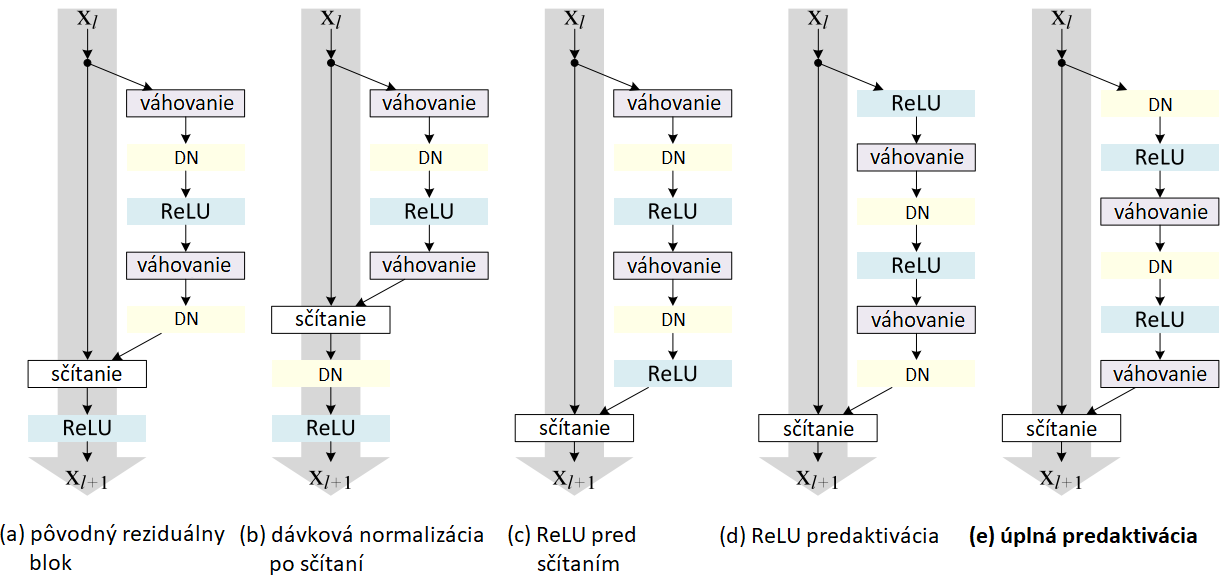
\includegraphics[width=1\textwidth]{images/architectures_of_residual_blocks}}
%popis obrazku
\caption[Vizualizácia rôznych architektúr reziduálnych blokov]{Vizualizácia rôznych architektúr reziduálnych blokov. Jednotlivé architektúry demonštrujú kombinácie operácií ktoré vykonávajú kumulované vrstvy za účelom transformácie dát $x_l$ (dávková normalizácia (DN), váhovanie, ReLU) \cite{He2016}.}
\label{fig:architectures_of_residual_blocks}
%id obrazku, pomocou ktoreho sa budeme na obrazok odvolavat
\end{figure}

Identitné prepojenie môže vykonať transformáciu identického zobrazenia šíreného týmto prepojením. Transformácia identického zobrazenia prechodom identitným prepojením má signifikantne veľký vplyv na výsledok predikcie reziduálnej siete \cite{He2016}. Pozorovanie preukázalo, že najkvalitnejšie predikcie poskytovala architektúra reziduálneho bloku \textbf{bez} transformácie identického zobrazenia šíreného identitným prepojením (viď Obrázok \ref{fig:achitectures_of_identity_shortcut} a)) \cite{He2016}. Ďalšie výsledky pozorovaní vplyvu architektúry identitného prepojenia na kvalitu predikcie reziduálnej siete je možné vidieť v tabuľke v Prílohe \ref{compareIdentityTransformations}

\begin{figure}
%vlozenie samotneho obrazku vycentrovaneho a vhodnej velkosti
%obrazok je v subore images/cervik.png
\centerline{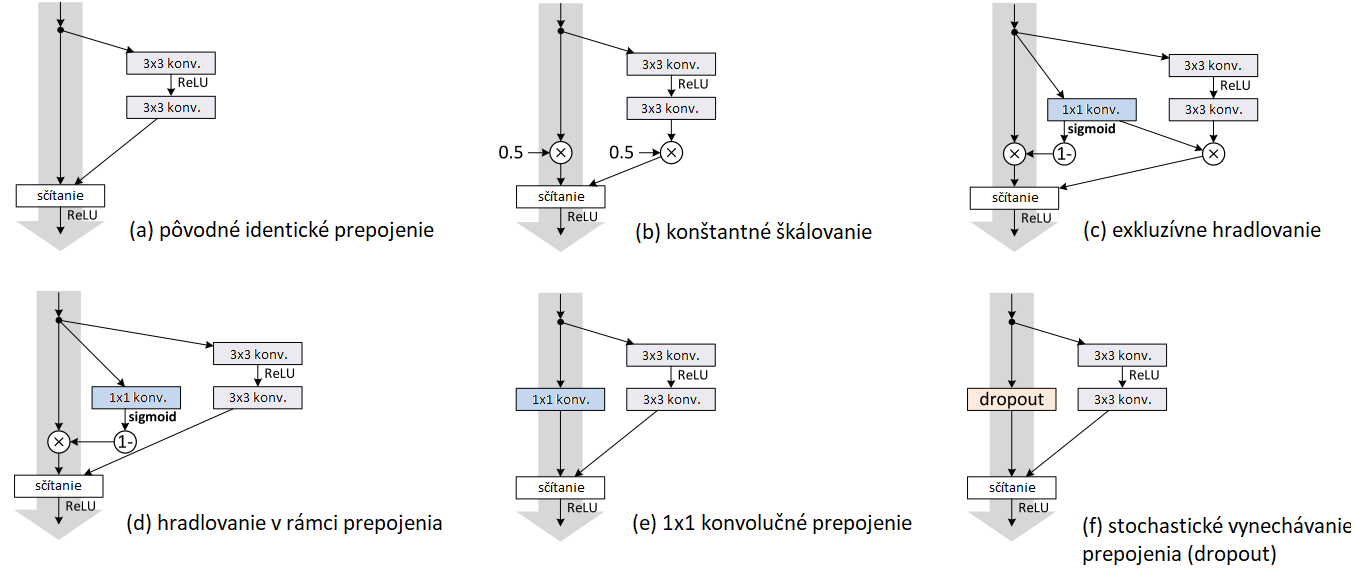
\includegraphics[width=1\textwidth]{images/achitectures_of_identity_shortcut}}
%popis obrazku
\caption[Vizualizácia rôznych architektúr identitneho prepojenia]{Vizualizácia rôznych architektúr identitného prepojenia. Pre zjednodušenie sme zanedbali operácie vykonávané v kumulovaných vrstvách \cite{He2016}.}
\label{fig:achitectures_of_identity_shortcut}
%id obrazku, pomocou ktoreho sa budeme na obrazok odvolavat
\end{figure}



\section{Zhrnutie reziduálnych sieti}
\label{conclusionResNet}

Reziduálne siete sú schopné predikovať identické zobrazenie \cite{Wu2017, He2016, Targ2016}. Na predikciu identického zobrazenia, reziduálne siete využívajú reziduálne bloky. Reziduálne bloky obsahujú niekoľko kumulovaných vrstiev a identitné prepojenie ktoré šíri identické zobrazenie obdržané daným reziduálnym blokom. Na výstupe reziduálneho bloku sa dané identické zobrazenie sčítava s transformovanou verziou toho istého identického zobrazenia (viď obrázok \ref{fig:residualBlock}). Transformácia identického zobrazenia je realizovaná kumulovanými vrstvami, ktoré nad obdržaným identickým zobrazením vykonávajú dávkovú normalizáciu, váhovanie a nelineárnu transformáciu.

Vzhľadom k tomu, že reziduálne bloky disponujú identitným prepojením, tak pre celú reziduálnu sieť je jednoduchšie aproximovať reziduálnu funkciu $\mathcal{F}(x)$ ako pomocou viacerých jednoduchých vrstiev aproximovať identitnú funkciu $\mathcal{H}(x)$. V prípade veľmi hlbokých neurónových sieti vzniká jav zvaný \textit{miznúci gradient}. Tento jav spôsobuje degradáciu presnosti neurónovej siete. V prípade \textit{miznúceho gradientu} dochádza k situácii kedy presnosť neurónovej siete prestane konvergovať a začne sa rapídne znižovať. Zavedením identitných prepojení do celého modelu neurónovej siete je možné tomuto javu predchádzať. Vďaka identitným prepojeniam je možné trénovať aj modely so sto až tisíc skrytými vrstvami a to bez výskytu degradácie presnosti \cite{Wu2017}.

Reziduálne siete nadobudli veľký rozmach, keďže experimenty potvrdili, že sú schopné úspešne predikovať identitu aj s využitím veľkého množstva skrytých vrstiev. Na súťaži ILSVRC 2015, získala 1. miesto implementácia reziduálnej siete, ktorá vykonávala klasifikáciu s chybou len 3.57\%. Na súťaži ILSVRC a COCO 2015, získala 1. miesto implementácia reziduálnej siete ktorá vykonávala detekciu, lokalizáciu a segmentáciu obrazu \cite{Wu2017}.

V našom prípade sú reziduálne siete ideálnym prostriedkom na skúmanie vplyvu syntetického gradientu na neurónové siete. Ako sme uviedli v kapitole \ref{residual_learning}, aj neurónová sieť využívajúca identitné prepojenia na šírenie identického zobrazenia (reziduálna sieť) upravuje svoje váhy pomocou gradientu šíreného spätnou propagáciou chyby. Zdroj \cite{Jaderberg2016} uvádza, že akákoľvek neurónová sieť ktorá využíva gradient šírený spätnou propagáciou chyby na úpravu svojich váh je schopná využívať na úpravu svojich váh aj syntetický gradient. Z týchto tvrdení usudzujeme, že implementácia syntetického gradientu v reziduálnych sieťach by nemala mať signifikantné negatívny vplyv na presnosť danej reziduálnej siete.